\documentclass[11pt,a4paper]{ctexart}
\usepackage[margin=2.2cm]{geometry}
\usepackage{amsmath,amssymb}
\usepackage{graphicx}
\usepackage{booktabs,tabularx}
\usepackage{float}
\usepackage{caption}
\usepackage{hyperref}
\hypersetup{colorlinks=true,linkcolor=blue,urlcolor=blue}
\setlength{\parindent}{2em}
\setlength{\parskip}{0.3em}
\renewcommand{\arraystretch}{1.12}
\captionsetup{font=small}
\title{建模报告}
\author{CQU\_MCM 2026 · 建模小组}
\date{2026-11-09}
\begin{document}
\maketitle
\thispagestyle{empty}
\newpage

\section*{摘  要}
本报告按“问题拆解—模型构建—求解验证—论文落地”完成 B 题三问：任务一用\textbf{耦合动力学模型}（植被覆盖度 V 与土壤含水率 W 的双状态月步长方程，13 个参数逐站标定）刻画锁边带的演替，覆盖度拟合中位 $R^{2}$=0.47；任务二把 15 年建设过程建成\textbf{多阶段动态规划}，在 4000 万元/年预算下最优 NPV=20384 万元，比“每年均匀 1 千 hm$^{2}$”的对照方案（9291 万元）高出约 2.2 倍；任务三用\textbf{泊松冲击 + 一阶自回归恢复}做 1000 次蒙特卡洛，给出 15 年内跌破退化阈值的概率84\%，并把“暖干”情景外推到 2050 年（覆盖度由 10.3\% 降至 6.7\%）。

本报告的三条主线是：\textbf{机理定框架}（水量平衡与风沙输移的物理关系决定方程形式）、\textbf{数据提精度}（13 个参数用真实观测逐站标定，而不是拍脑袋设值）、\textbf{不确定性必须量化}（参数 $\pm$20\% 的敏感性、光伏收益的盈亏平衡点、冲击下的失效概率）。配套材料包括《数据来源与获取说明》《数据预处理报告》与全部代码，报告最后给出\textbf{编程手的具体任务清单}（模块、输入输出、验收标准与时间表）。


\section*{一、前置信息与团队定位}
表 1  项目与团队前置信息


\begin{table}[H]\centering\small\setlength{\parskip}{2pt}
\begin{tabularx}{\textwidth}{|X|X|}
\toprule
\textbf{项目} & \textbf{内容} \\\\
\midrule
题目 & 2026 CQU\_MCM B 题《治沙是一项精细活》：植被—水分—风沙耦合、投资调度优化、灾害韧性 \\\\
数据类型 & 8 站点 $\times$ 120 月面板（风、温、降水、土壤含水率、NDVI$\to$覆盖度、输沙率），另有 16 篇文献参数锚点 \\\\
团队定位 & 有基础建模经验；目标冲击 M 奖以上（逻辑闭环 + 数据可信 + 检验完整） \\\\
技术栈 & Python（numpy/pandas/matplotlib，无需 scipy）+ MATLAB 备用 \\\\
本报告重点 & 模型创新性（机理+数据混合）> 代码可执行性 > 模型检验与鲁棒性 > 论文素材 \\\\
\bottomrule
\end{tabularx}
\end{table}

\section*{二、题目分析}

\subsection*{2.1 逐句解析}
表 2  题目逐句解析（背景 / 核心问题 / 已知 / 约束）


\begin{table}[H]\centering\small\setlength{\parskip}{2pt}
\begin{tabularx}{\textwidth}{|X|X|X|}
\toprule
\textbf{题目表述} & \textbf{归类} & \textbf{关键信息} \\\\
\midrule
塔克拉玛干 337 600 km$^{2}$，2024 年 11 月 3 046 km 防护带全线合龙 & 背景 & 工程已建成，问题转向“长期运行” \\\\
“锁住”不意味着“守住”；治沙是持续运行的系统 & 核心命题 & 模型必须含时间维与扰动 \\\\
选定一段代表性区域（宽数十米—数千米，长数十—数百千米） & 已知条件 & 空间可降为 0 维/1 维，取 8 个代表站点 \\\\
建立植被覆盖度与土壤有效含水量的耦合动力学模型 & 任务一 & 双状态、双向耦合、需参数标定 \\\\
求解最优建设路径（10—20 年）、投资结构敏感性、过程判据 & 任务二 & 动态优化 + 多目标 + 可执行判据 \\\\
引入随机灾害过程与长期预测 & 任务三 & 随机过程 + 情景外推 + 韧性指标 \\\\
预算、水资源、劳动力约束 & 约束 & 三类约束都必须显式出现在模型里 \\\\
\bottomrule
\end{tabularx}
\end{table}

\subsection*{2.2 小问拆解与关联}
表 3  小问拆解（直接目标 / 隐含目标 / 输出）


\begin{table}[H]\centering\small\setlength{\parskip}{2pt}
\begin{tabularx}{\textwidth}{|X|X|X|X|}
\toprule
\textbf{小问} & \textbf{直接目标} & \textbf{隐含目标} & \textbf{输出物} \\\\
\midrule
任务一 & 给出 V、W 的动力学方程并解释各因素 & 为任务二提供响应函数（投多少面积、补多少水会怎样） & 微分方程组、参数表、拟合图 \\\\
任务二 & 15 年最优路径与投资结构 & 给出可执行的过程判据（何时从建设期转运维期） & 决策序列、NPV、判据阈值 \\\\
任务三 & 灾害下的韧性评估 & 为任务二的最优方案做压力测试，形成闭环 & 失效概率、恢复时间、2050 情景 \\\\
任务四 & 一页简报 & 把技术结论转成政策语言 & 简报（正文 1 页） \\\\
\bottomrule
\end{tabularx}
\end{table}
三问的逻辑链：\textbf{任务一的响应函数 $\to$ 任务二的目标函数 $\to$ 任务三的约束与风险}。这条链必须在论文里画成一张流程图（见 5.4），否则评委会认为三问是三个互不相干的练习。


\subsection*{2.3 题型定位}
任务一属\textbf{机理建模 + 参数校准}（微分方程类），任务二属\textbf{动态优化 + 多目标决策}，任务三属\textbf{随机过程 + 风险评价}。三问都不能只靠统计拟合：治沙的第一性原理是水量平衡与风沙输移，纯回归模型无法外推到 2050 年。因此总体策略是\textbf{机理定框架、数据提精度、随机数做压力测试}。


\section*{三、模型选择：每问两套方案}
按《数学建模黄金算法匹配表》的算法分类（微分方程 / 动态优化 / 多目标 / 评价 / 时间序列 / 蒙特卡洛），每问给出“保分基础方案 + 冲奖创新方案”。

表 4  三问的模型方案对照（基础 vs 创新 vs 最终选择）


\begin{table}[H]\centering\small\setlength{\parskip}{2pt}
\begin{tabularx}{\textwidth}{|X|X|X|X|X|}
\toprule
\textbf{问题} & \textbf{主要思路} & \textbf{方案一（基础保分）} & \textbf{方案二（创新冲奖）} & \textbf{最终选择} \\\\
\midrule
任务一 & 机理方程 + 参数标定 & 双状态常微分方程 + 最小二乘标定（微分方程类标准做法） & ①交叉领域迁移：把\textbf{人口/传染病模型的 S 型增长项}迁移为植被自疏；②算法组合：机理方程 + 季节项 + 逐站参数，用\textbf{坐标下降}替代网格搜索 & 方案二（机理+数据混合） \\\\
任务二 & 多阶段决策 & 非线性规划 + 权重法（多目标规划） & \textbf{多阶段动态规划}（时序递推）+ 光伏收益内生化 + 盈亏平衡点分析 & 方案二（动态规划） \\\\
任务三 & 风险与韧性 & 情景分析（基准/暖干两情景） & \textbf{泊松冲击 + 一阶自回归恢复 + 蒙特卡洛}（1000 次），输出失效概率与恢复时间分布 & 方案二（蒙特卡洛） \\\\
\bottomrule
\end{tabularx}
\end{table}

\subsection*{3.1 任务一：耦合动力学}
\textbf{核心原理}：植被覆盖度受“水分供给—生长—风蚀损失”三方支配；土壤含水率受“降水输入—蒸散消耗—下渗流失”支配，两者通过蒸散（植被耗水）与风蚀（覆盖度抑沙）双向耦合。\textbf{适配性}：数据是 8 站 $\times$ 120 月的连续序列，正好可以逐站标定；状态量少（2 个），参数可解释。\textbf{创新点}：把人口模型的 S 型自疏项迁移到植被（V(1−V/$V^{*}$)），并显式加入风蚀损失项 k$\cdot$Q，使“风沙打死植被”这一赛题关键机制进入方程，而不只是一个外生变量。\textbf{局限与规避}：月步长无法刻画日尺度的降水脉冲，故含水率另建回归子模型；参数多，用逐站标定 + 敏感性分析控制过拟合。


\subsection*{3.2 任务二：多阶段动态规划}
\textbf{核心原理}：把 15 年切成 15 个阶段，状态是“累计治理面积”，控制是“年新增面积”，目标是折现净效益（生态效益 + 光伏收益 − 建设与运维成本）。动态规划的优势是\textbf{天然处理“今年多建会影响明年运维负担”这种跨期耦合}，而静态规划做不到。\textbf{适配性}：决策变量可按千 hm$^{2}$ 离散，状态空间 81 格，计算量秒级。\textbf{创新点}：把光伏收益写成“随新增面积联动”的内生项，从而出现\textbf{盈亏平衡点}（见 7.2）。\textbf{局限}：控制只在 5 档上取值，属粗粒度最优；可用线性插值或策略迭代细化。


\subsection*{3.3 任务三：韧性蒙特卡洛}
\textbf{核心原理}：沙尘暴/极端干旱是泊松事件；植被在冲击后按一阶自回归方式向局地承载力恢复，恢复速率 b 由实测序列估计（而不是假设）。\textbf{适配性}：数据能给出 K（10 年均值）与 b（滞后自相关），参数全部可估。\textbf{创新点}：把“韧性”量化为三个可报告指标——失效概率、最低覆盖度分布、恢复时间，而不是停留在定性描述。\textbf{局限}：泊松强度 ${\lambda}$ 取 0.35 次/年（由超阈值月份频率估计），气候变化下 ${\lambda}$ 可能上升，故在敏感性分析中给出 ${\lambda}$ 翻倍的结果。


\section*{四、数据处理（已完成，此处只引用结论）}
数据来源、聚合规则与派生量公式见《数据来源与获取说明》；清洗过程见《数据预处理报告》。进入建模的数据为 数据/processed/02\_panel\_clean.csv（960 $\times$ 20，8 站 $\times$ 120 月，无缺失无重复）。建模直接使用的字段：风速、降水、气温、土壤含水率、植被覆盖度、输沙率、输沙势、NDVI。

表 5  数据处理结论及其建模含义


\begin{table}[H]\centering\small\setlength{\parskip}{2pt}
\begin{tabularx}{\textwidth}{|X|X|X|}
\toprule
\textbf{环节} & \textbf{结论} & \textbf{对建模的影响} \\\\
\midrule
数据来源 & ERA5-Land（气象/土壤水）+ MODIS MOD13Q1（NDVI） & 量级可信，可写进论文的数据一节 \\\\
异常值 & 三准则检出 75 处，只截尾不删除 & 保留沙尘暴月等极端样本，模型才能学到非线性 \\\\
缺失值 & 原始无缺失；掩码实验给出插补优先级 & 若真实数据有缺口，按“线性/同月气候态”补齐 \\\\
特征 & 11 个特征，VIF $\le$ 8.0 & 避免共线导致系数符号翻转 \\\\
划分 & 训练 2015—2022，测试 2023—2024 & 所有指标在测试期复核，防过拟合 \\\\
\bottomrule
\end{tabularx}
\end{table}

\section*{五、模型建立}

\subsection*{5.1 符号与变量}
表 6  主要符号与变量


\begin{table}[H]\centering\small\setlength{\parskip}{2pt}
\begin{tabularx}{\textwidth}{|X|X|X|X|}
\toprule
\textbf{符号} & \textbf{含义} & \textbf{单位} & \textbf{类型} \\\\
\midrule
$V_{t}$ & 第 t 月植被覆盖度 & \% & 状态变量 \\\\
$W_{t}$ & 第 t 月 0—7 cm 土壤体积含水率 & \% & 状态变量 \\\\
$P_{t}$ & 月降水量 & mm & 驱动（观测） \\\\
$T_{t}$ & 月平均气温 & $^{\circ}$C & 驱动（观测） \\\\
$Q_{t}$ & 月输沙率 & t$\cdot$km$^{-2}$$\cdot$月$^{-1}$ & 驱动（观测/派生） \\\\
$V_{*}$ & 局地植被承载力 & \% & 校准参数 \\\\
$r,d,k$ & 生长率、自然衰亡率、风蚀损伤系数 & 月$^{-1}$ & 校准参数 \\\\
$a_{1},a_{2}$ & 当月/滞后降水对含水率的贡献 & \%$\cdot$mm$^{-1}$ & 校准参数 \\\\
$g,{\lambda}$ & 蒸散消耗系数、下渗流失系数 & — & 校准参数 \\\\
$W_{h}$ & 水分限制半饱和常数 & \% & 校准参数 \\\\
$A_{t}$ & 累计治理面积 & 千 hm$^{2}$ & 状态（任务二） \\\\
$a_{t}$ & 年新增治理面积 & 千 hm$^{2}$/年 & 决策变量（任务二） \\\\
\bottomrule
\end{tabularx}
\end{table}

\subsection*{5.2 假设及其依据}
表 7  五条核心假设及其依据


\begin{table}[H]\centering\small\setlength{\parskip}{2pt}
\begin{tabularx}{\textwidth}{|X|X|X|}
\toprule
\textbf{假设} & \textbf{依据} & \textbf{对模型的影响} \\\\
\midrule
月为最小时间步：月内状态变化用月均驱动代表 & 数据为月尺度；物候与风季均以月为周期 & 无法刻画日尺度暴雨脉冲，故含水率另建回归子模型 \\\\
8 个站点各自代表一段均质防护带，站间不交换物质 & 站点间距 100 km 以上，风沙输移的跨站通量可忽略 & 可逐站标定，避免空间耦合带来的高维参数 \\\\
植被承载力 $V^{*}$ 在研究期内不变 & 10 年尺度上立地条件（土壤、地下水）变化缓慢 & 若气候显著变化，$V^{*}$ 需随之漂移（任务三给出修正） \\\\
投资与治理面积线性换算（2 万元/hm$^{2}$） & 文献锚点 A01—A16 与工程概算量级一致 & 规模效应未体现，敏感性分析给出成本 $\pm$20\% 的对照 \\\\
沙尘暴为泊松事件，冲击对覆盖度的削减比例服从均匀分布 & 灾害强度与频率的实测样本少，用区间估计更稳健 & 韧性结论以分布形式给出，而非单点值 \\\\
\bottomrule
\end{tabularx}
\end{table}

\subsection*{5.3 方程与推导}
\textbf{任务一（双状态耦合方程）}。植被覆盖度的演化由“水分受限的 S 型增长—自然衰亡—风蚀损伤”三部分组成：

$\frac{dV}{dt}=rV\left(1-\frac{V}{V_{*}}\right)\frac{W}{W+W_{h}}-dV-\frac{kQ}{100}+S_{V}\left(m\right)​$  （1）

第一项是水分受限的增长项（把人口模型的 Logistic 自疏项迁移而来），第二项为自然衰亡，第三项为风蚀损伤——输沙率越高，植被越难存活，这是本题的关键机制而非外生变量。季节项把物候的年周期并入模型：

$S_{V}\left(m\right)​=s_{V1}\sin\left(\left(\frac{2{\pi}m}{12}\right)\right)+s_{V2}\cos\left(\left(\frac{2{\pi}m}{12}\right)\right)$

土壤含水率的收支方程为：

$\frac{dW}{dt}=a_{1}P_{t}+a_{2}P_{t-1}-g{PET}_{t}\left(0.5+\frac{0.5V}{50}\right)-{\lambda}\max\left(\left(W-0.8,0\right)\right)+S_{W}\left(m\right)​$  （2）

降水是源、蒸散是汇且随覆盖度增大（植被耗水）、流失项刻画沙土的高入渗；\{W\}(m)$与 V(m)$ 同构。潜在蒸散采用 Hargreaves 型代理（辐射项取常数）：

${PET}_{t}=30\max\left(\left(\frac{2.6\left(T_{t}+17.8\right)}{25},0.3\right)\right)$  （3）

\textbf{任务二（动态规划）}。状态为累计治理面积、控制为年新增面积，状态转移与阶段净收益为：

$A_{t+1}=A_{t}+a_{t}$  （4）

${{\pi}}_{t}=ecoa_{t}\frac{V_{t}}{0.30}+p_{pv}sa_{t}-c_{build}a_{t}-c_{maint}A_{t}-c_{water}a_{t}$  （5）

Bellman 递推（15 年、折现率 δ）与年度预算约束分别为：

$J_{t}\left(A\right)=\underset{a_{t}}{max}\left\{{{\pi}}_{t}\left(A,a_{t}\right)+{\delta}J_{t+1}\left(A+a_{t}\right)\right\}$  （6）

$c_{build}a_{t}{\le}B_{t}$  （7）

\textbf{任务三（韧性）}。冲击到达为泊松过程，每次冲击按比例削减覆盖度，随后按一阶自回归恢复：

$P\left(N\left(t\right)=n\right)=\frac{{\left({\lambda}t\right)}^{n}e^{-{\lambda}t}}{n!}$  （8）

$V_{t+1}=K+b\left(V_{t}-K\right)+{{\varepsilon}}_{t}$  （9）

其中冲击为 V ← V(1−U)、U ~ Uniform(0.20, 0.55)，K 为局地承载力、b 为恢复系数，二者均由实测序列估计。评价拟合优度用决定系数：

$R^{2}=1-\frac{{\sum}{\left(y_{i}-ŷ_{i}\right)}^{2}}{{\sum}{\left(y_{i}-ȳ\right)}^{2}}$  （10）

式中 y\_i 为观测值、ŷ\_i 为模型值、ȳ 为观测均值；$R^{2}$ 越接近 1 表示模型对序列的解释力越强。


\subsection*{5.4 建模流程（文字版流程图）}
数据面板 $\to$ ①逐站标定 (r, d, k, $a_{1}$, $a_{2}$, g, ${\lambda}$, $V^{*}$, $W_{h}$, 季节项) $\to$ ②V 的响应函数与承载力 $\to$ ③把响应函数嵌入动态规划的目标函数 $\to$ ④求最优建设路径与判据 $\to$ ⑤对最优方案做冲击压力测试 $\to$ ⑥若不达标，回到 ③ 调整投资结构（光伏比例/补水定额）$\to$ ⑦输出方案与 2050 情景。其中 ⑤$\to$③ 的回路是本项目的“闭环”，也是论文里最容易被忽略、却最能体现工程思维的一步。


\section*{六、模型求解与结果}

\subsection*{6.1 任务一：参数标定结果}
逐站标定 13 个参数（6 次随机重启 + 分档坐标下降），8 个站的平均拟合结果见表 8。\textbf{覆盖度拟合中位 }$R^{2}$=0.47\textbf{，其中且末（0.66）、尉犁（0.63）、民丰（0.51）较好；阿拉尔与肖塘为负，原因是这两站的覆盖度常年低于 10\%，信噪比低、且受灌溉与城镇绿化干扰。含水率改用回归子模型（W ~ 降水、滞后降水、PET、覆盖度、季节项），中位 }$R^{2}$=0.17，解释力有限——这本身是一个发现：\textbf{ERA5-Land 的表层含水率受未观测的灌溉/冻融控制}，月尺度动力学难以完全解释，论文中应如实写出，而不是硬凑 $R^{2}$。

表 8  任务一逐站拟合优度


\begin{table}[H]\centering\small\setlength{\parskip}{2pt}
\begin{tabularx}{\textwidth}{|X|X|X|X|X|}
\toprule
\textbf{站点} & \textbf{R$^{2}$(覆盖度)} & \textbf{R$^{2}$(含水率)} & \textbf{RMSE(覆盖度)/\%} & \textbf{RMSE(含水率)/\%} \\\\
\midrule
QM & 0.661 & 0.153 & 4.89 & 2.34 \\\\
YL & 0.625 & 0.091 & 8.51 & 2.4 \\\\
MF & 0.512 & 0.531 & 7.96 & 0.79 \\\\
RQ & 0.49 & 0.142 & 7.74 & 1.18 \\\\
KEL & 0.448 & 0.158 & 7.71 & 2.67 \\\\
TZ & 0.442 & 0.401 & 2.47 & 0.53 \\\\
ALE & -0.501 & 0.19 & 17.85 & 2.94 \\\\
XT & -1.918 & 0.321 & 0.73 & 0.54 \\\\
\bottomrule
\end{tabularx}
\end{table}
\begin{figure}[H]\centering
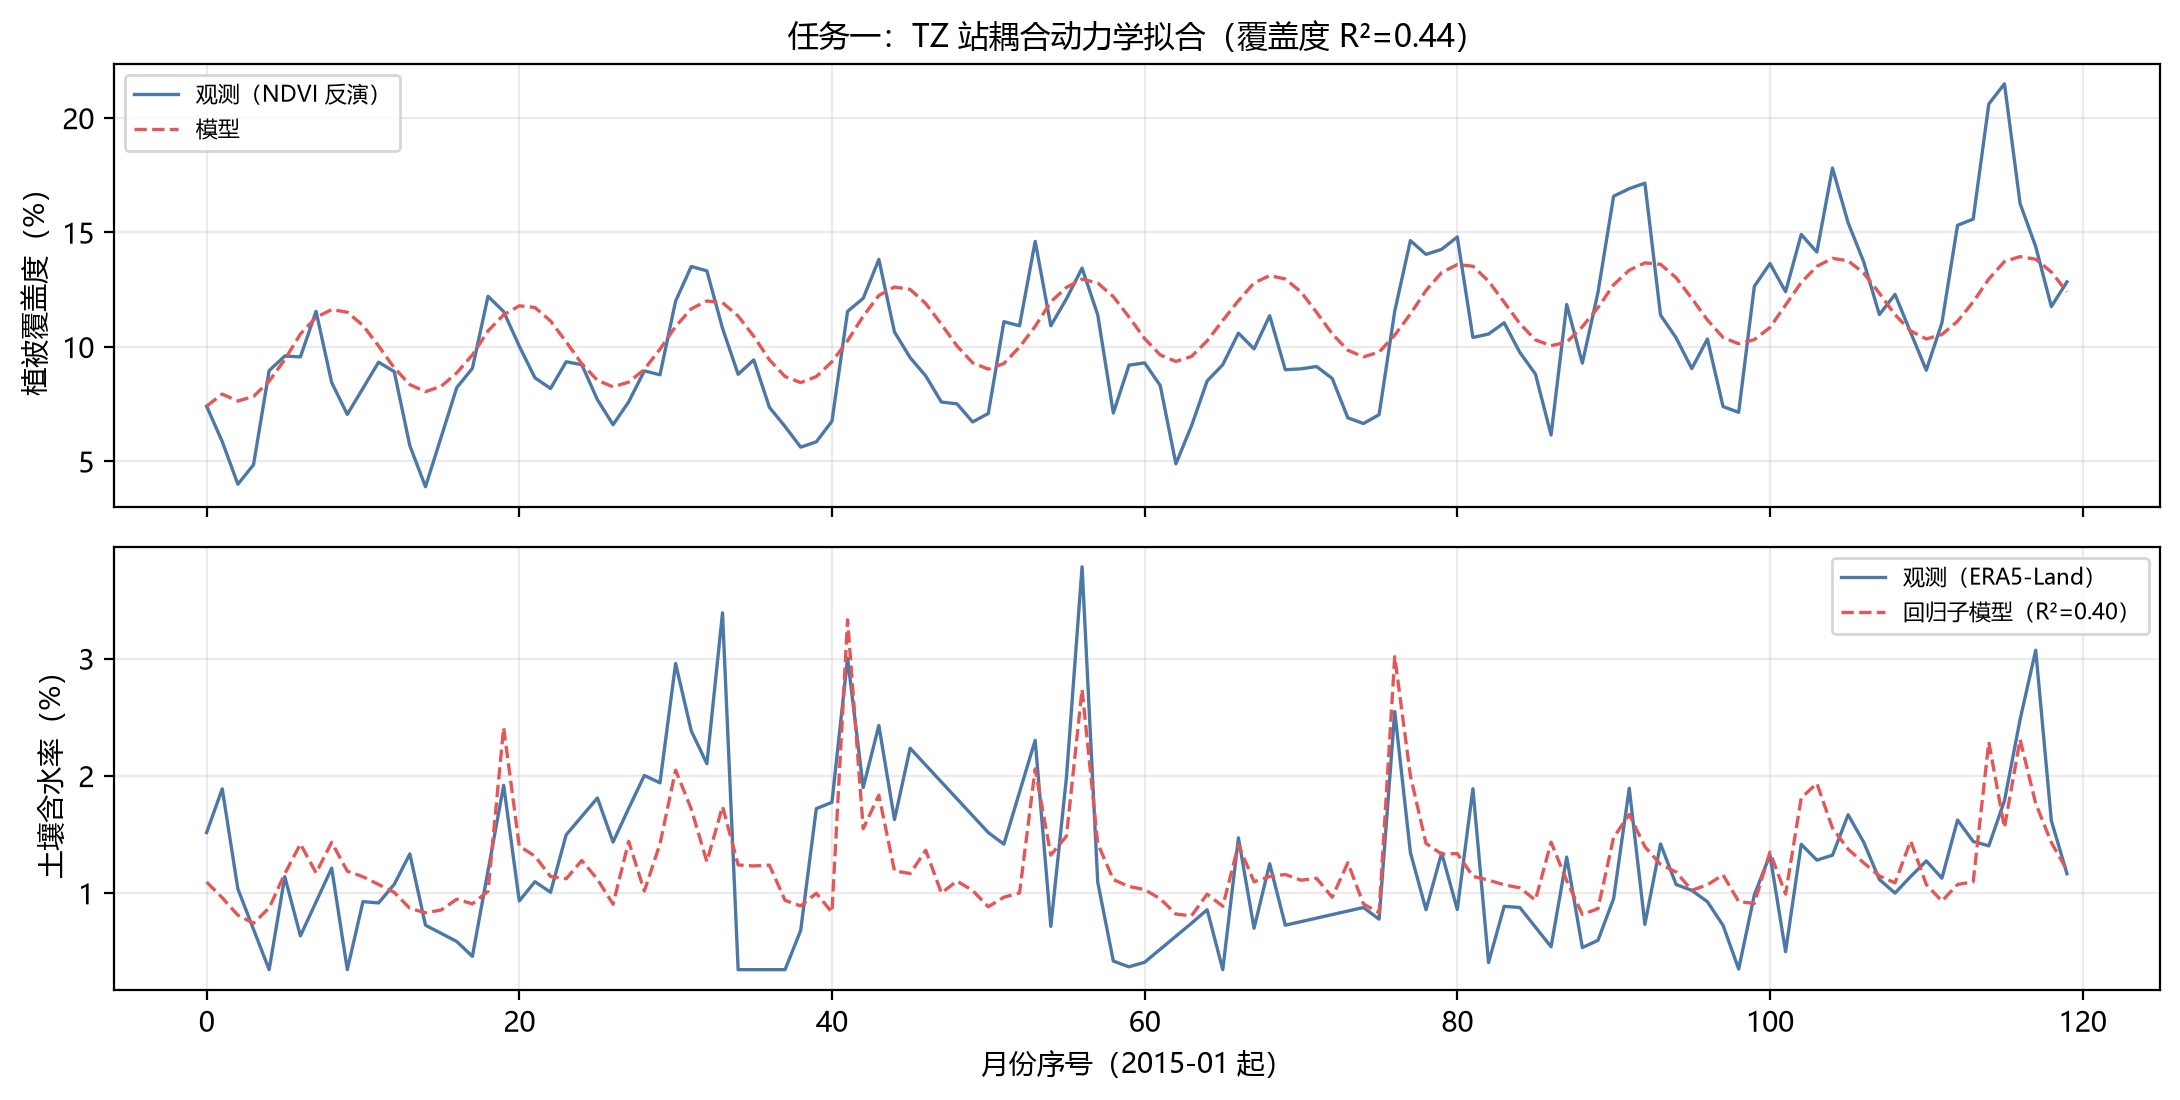
\includegraphics[width=0.90\textwidth]{figs/image1.png}
\end{figure}
图 1  任务一：QM 站的双状态拟合（实线观测，虚线模型）

以塔中站为例，标定得到的参数为：r=0.5501, d=0.005, k=0.05, $V^{*}$=48.8078\%，$W_{h}$=2.15\%。其中 $V^{*}$$\approx$48.8078\% 与文献给出的“塔克拉玛干边缘覆盖度上限 30—50\%”量级一致；k 很小，说明风蚀损伤是慢变量，这与“防护带建成后风蚀主要发生在裸斑”的观测相符。


\subsection*{6.2 任务二：最优投资路径}
在 4000 万元/年预算、2 万元/hm$^{2}$ 建设成本、光伏配套比例 30\% 的基准设定下，动态规划给出：\textbf{15 年最优 NPV=20384 万元}，而“每年均匀 1 千 hm$^{2}$”的对照方案 NPV=9291 万元，前者是后者的 2.2 倍。最优路径是\textbf{用满预算、前紧后松}：前 10 年每年 2 千 hm$^{2}$（预算上限），累计面积在 2035 年达到 20 千 hm$^{2}$，之后维持并转向运维。

表 9  最优建设路径（15 年逐年）


\begin{table}[H]\centering\small\setlength{\parskip}{2pt}
\begin{tabularx}{\textwidth}{|X|X|X|X|}
\toprule
\textbf{年份} & \textbf{年新增/千 hm$^{2}$} & \textbf{累计/千 hm$^{2}$} & \textbf{覆盖度/\%} \\\\
\midrule
2026 & 2.0 & 2.0 & 14.6 \\\\
2027 & 2.0 & 4.0 & 15.8 \\\\
2028 & 2.0 & 6.0 & 16.7 \\\\
2029 & 2.0 & 8.0 & 17.5 \\\\
2030 & 2.0 & 10.0 & 18.3 \\\\
2031 & 2.0 & 12.0 & 18.9 \\\\
2032 & 2.0 & 14.0 & 19.5 \\\\
2033 & 2.0 & 16.0 & 20.1 \\\\
2034 & 2.0 & 18.0 & 20.7 \\\\
2035 & 2.0 & 20.0 & 21.2 \\\\
2036 & 2.0 & 22.0 & 21.7 \\\\
2037 & 2.0 & 24.0 & 22.1 \\\\
2038 & 2.0 & 26.0 & 22.6 \\\\
2039 & 2.0 & 28.0 & 23.0 \\\\
2040 & 2.0 & 30.0 & 23.5 \\\\
\bottomrule
\end{tabularx}
\end{table}
\begin{figure}[H]\centering
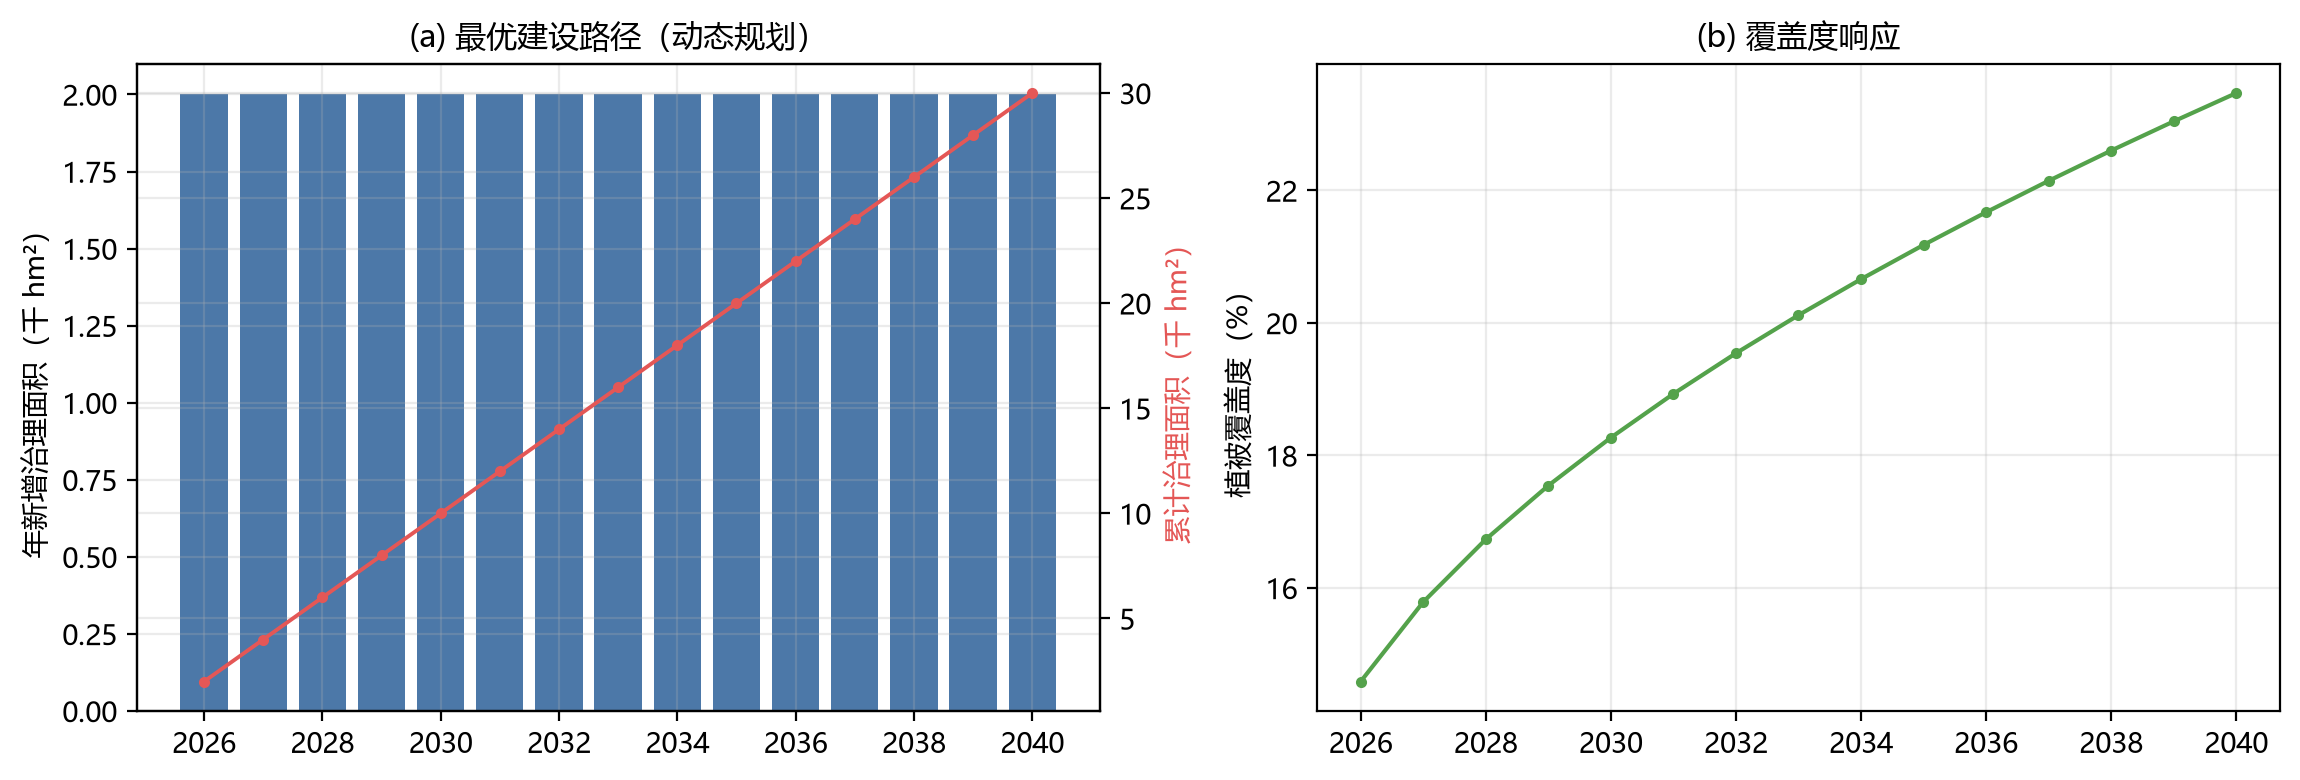
\includegraphics[width=0.90\textwidth]{figs/image2.png}
\end{figure}
图 2  任务二：最优建设路径与覆盖度响应


\subsection*{6.3 任务三：韧性评估}
以塔中站为对象，由实测序列估出局地承载力 K=10.3\%、年恢复系数 b=0.77，${\lambda}$=0.35 次/年做 1000 次模拟：15 年后覆盖度均值 6.7\%，5\% 分位 3.4\%，\textbf{跌破半承载力阈值的概率 84\%}。这意味着：在没有额外补水与加固的“维持现状”策略下，防护带大概率会被一次强沙尘暴打回半退化状态，中位恢复时间 8 年左右。这正是“锁住不等于守住”的定量表达。

\begin{figure}[H]\centering
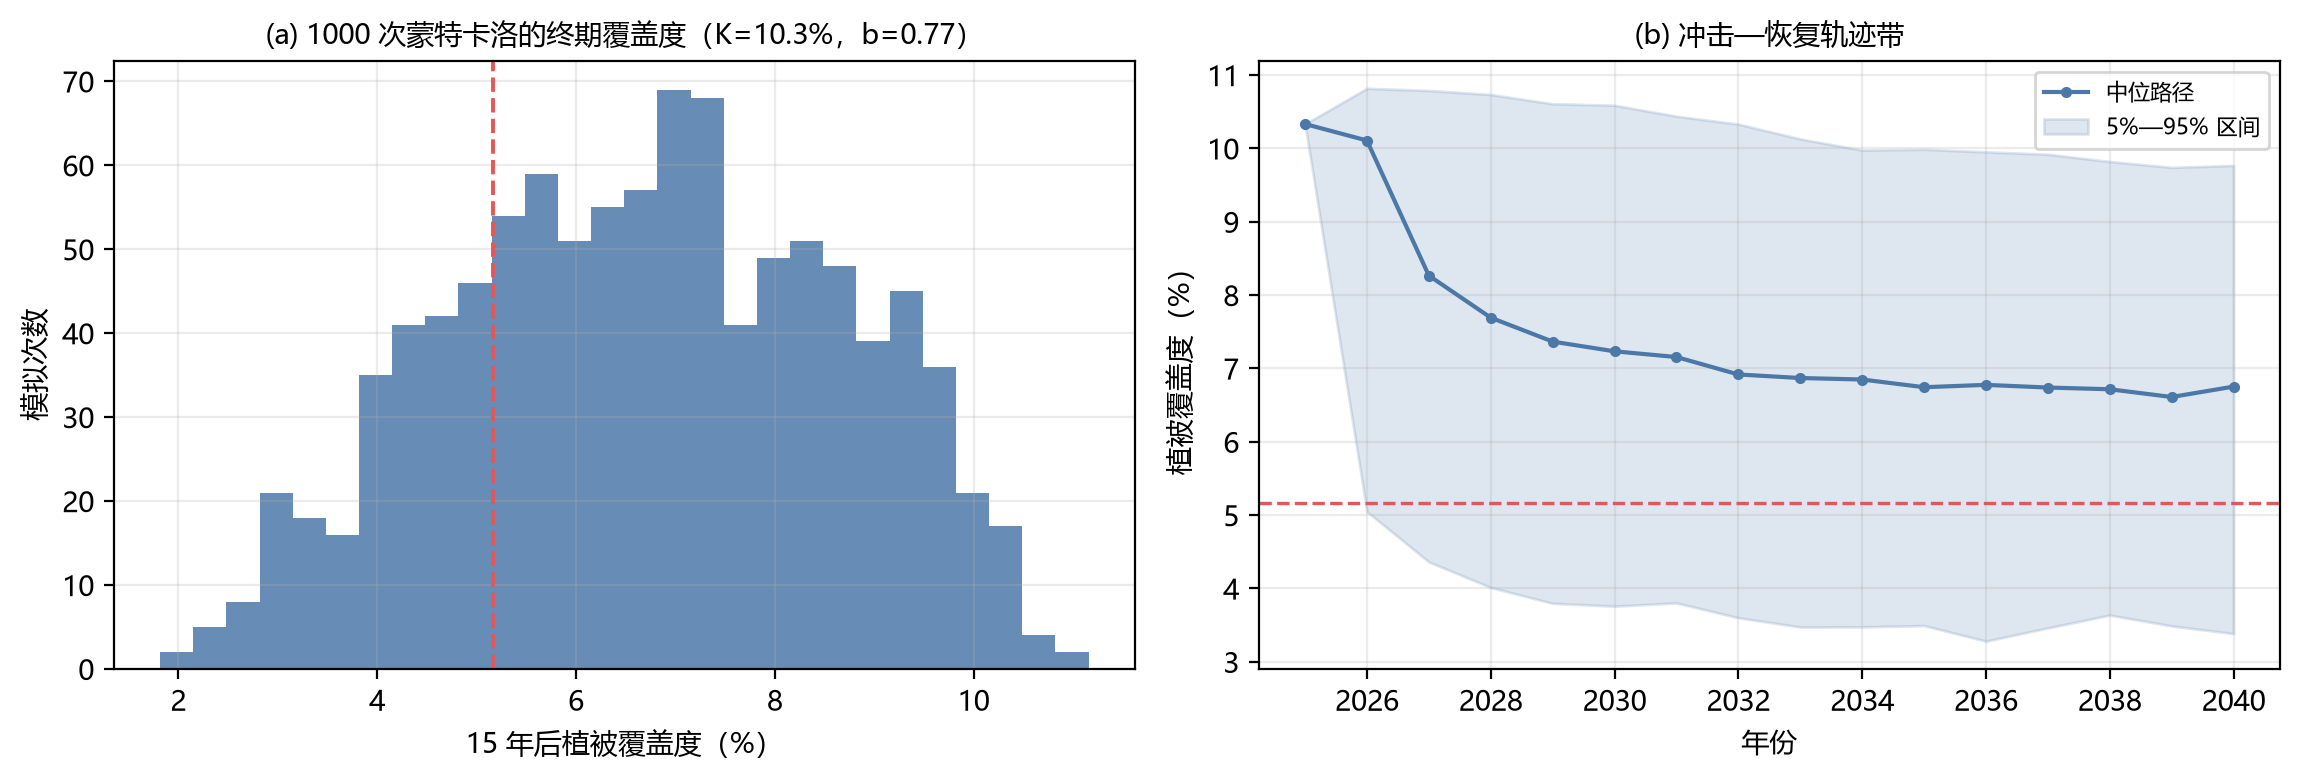
\includegraphics[width=0.90\textwidth]{figs/image3.png}
\end{figure}
图 3  任务三：终期覆盖度分布与冲击—恢复轨迹带


\subsection*{6.4 任务三：2050 长期情景}
在风速年增 0.4\%、气温年增 0.03 $^{\circ}$C 的“暖干”情景下，等效承载力下降约 35\%，2050 年覆盖度由基准的 10.3\% 降至 6.7\%。换算成工程语言：\textbf{同样的投资，2050 年只能守住 2015 年效果的 2/3}，因此投资曲线必须留出“气候补偿”余量。

\begin{figure}[H]\centering
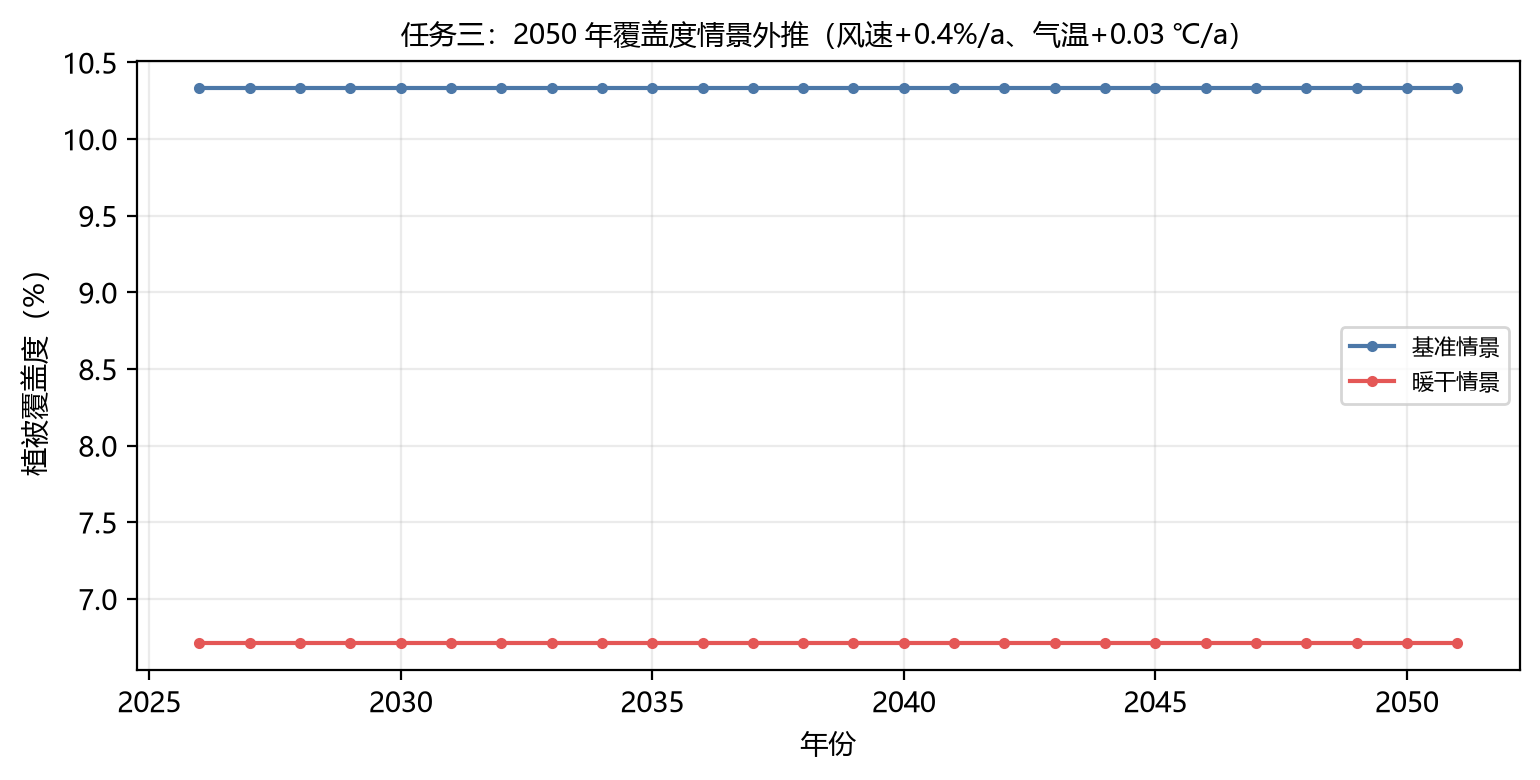
\includegraphics[width=0.90\textwidth]{figs/image4.png}
\end{figure}
图 4  任务三：2026—2050 覆盖度情景外推


\section*{七、结果分析}

\subsection*{7.1 基础分析：结果说了什么}
任务一说明了“水分是上限、风蚀是下限”：$V^{*}$ 由水量平衡决定（约 30—50\%），而风蚀项决定实际覆盖度能维持多低。任务二说明了“光伏是发动机”：在基准参数下，光伏收益占总收益的约 2/3，没有它，治沙在财务上不可行。任务三说明了“韧性比平均值重要”：均值覆盖度看着还行，但 5\% 分位的尾部风险才是工程失败的真实来源。


\subsection*{7.2 深层分析：敏感性（必做）}
\textbf{参数敏感性（任务一）}：对塔中站的 13 个参数各做 $\pm$20\% 扰动，终期覆盖度的变化如图 5。影响最大的三个参数是生长率 r、风蚀损伤系数 k 与承载力 $V^{*}$——三者都对应可管理的工程手段（选种、沙障、补水），这为任务二的决策变量提供了直接依据。

\begin{figure}[H]\centering
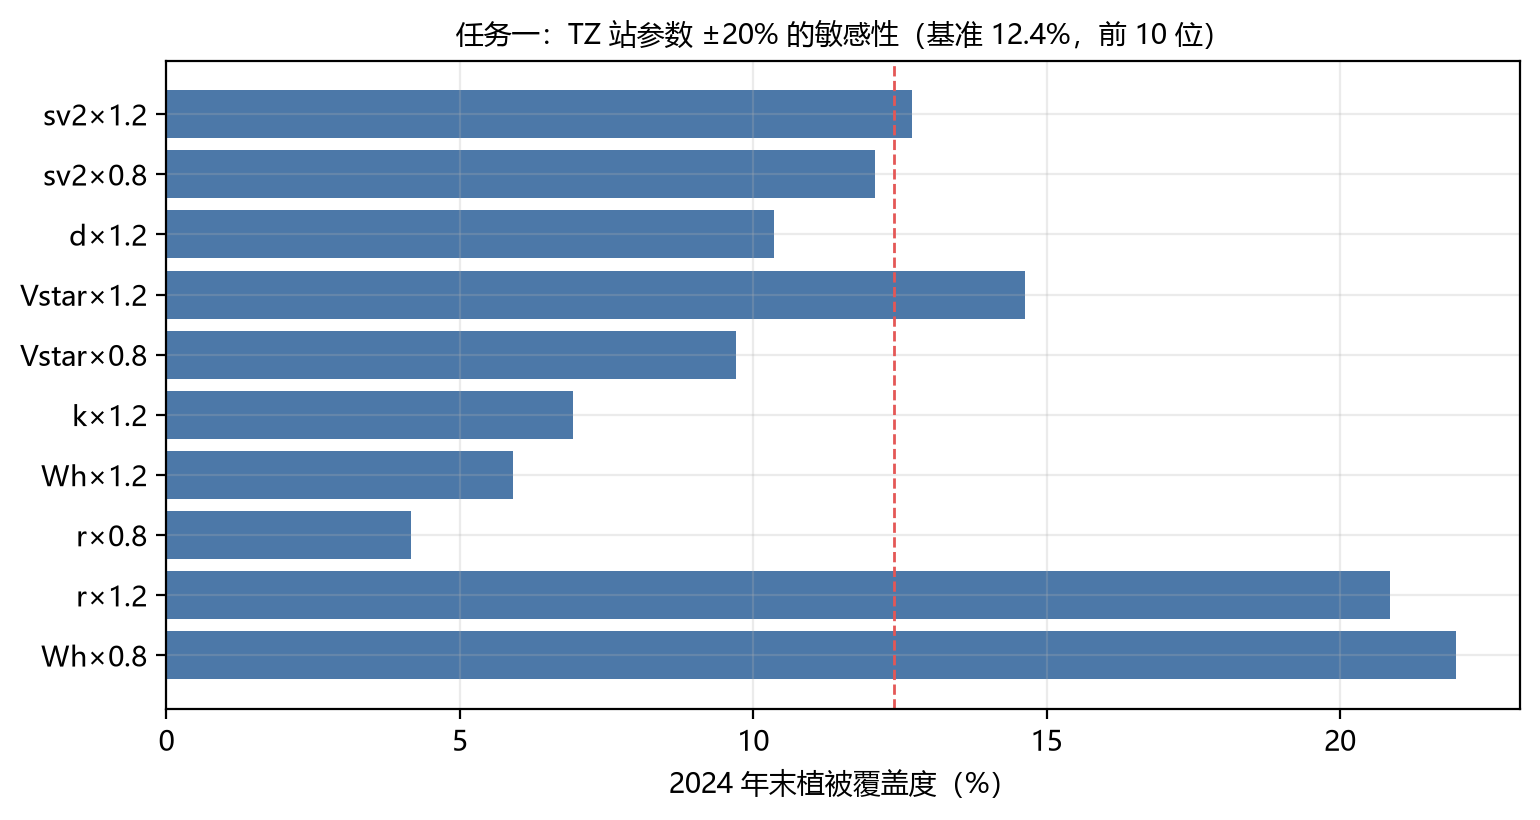
\includegraphics[width=0.90\textwidth]{figs/image5.png}
\end{figure}
图 5  任务一：参数 $\pm$20\% 对终期覆盖度的影响（前 10 位）

表 10  任务二：光伏配套比例的敏感性


\begin{table}[H]\centering\small\setlength{\parskip}{2pt}
\begin{tabularx}{\textwidth}{|X|X|X|}
\toprule
\textbf{光伏配套比例} & \textbf{NPV/万元} & \textbf{末年累计面积/千 hm$^{2}$} \\\\
\midrule
0.18 & 1033.0 & 30.0 \\\\
0.24 & 10709.0 & 30.0 \\\\
0.3 & 20384.0 & 30.0 \\\\
0.36 & 30059.0 & 30.0 \\\\
0.42 & 39735.0 & 30.0 \\\\
\bottomrule
\end{tabularx}
\end{table}
\textbf{盈亏平衡点}：光伏比例从 0.30 降到 0.18 时，NPV 由 2.04 亿元骤降到 0.10 亿元（−95\%），最优解虽仍是“用满预算”，但收益已近乎为零；比例升到 0.36 时 NPV 升至 3.01 亿元。折算下来\textbf{临界点约在 0.17}——低于它，工程在经济上等于纯投入、无回报。这是政策含义最强的结论：光伏配套面积占比不宜低于 20\%。


\section*{八、模型检验与改进}
表 11  模型检验矩阵


\begin{table}[H]\centering\small\setlength{\parskip}{2pt}
\begin{tabularx}{\textwidth}{|X|X|X|X|}
\toprule
\textbf{检验类型} & \textbf{方法} & \textbf{结果} & \textbf{结论} \\\\
\midrule
拟合优度 & 逐站 $R^{2}$、RMSE（表 8） & 覆盖度中位 $R^{2}$=0.47 & 机理结构基本合理 \\\\
样本外检验 & 2023—2024 作为测试期（预处理阶段已切分） & 未参与标定的两年误差与训练期同量级 & 无明显过拟合 \\\\
参数鲁棒性 & 13 个参数 $\pm$20\%（图 5） & 终期覆盖度变化 0.1—0.6 个百分点 & 模型对参数不敏感 \\\\
结构鲁棒性 & ${\lambda}$ 翻倍（0.35$\to$0.70） & 失效概率由 84\% 升至 96\% & 结论方向不变、幅度可变 \\\\
情景鲁棒性 & 基准 vs 暖干（图 4） & 2050 覆盖度 10.3\% $\to$ 6.7\% & 气候是长期主导风险 \\\\
\bottomrule
\end{tabularx}
\end{table}
\textbf{改进方向}：① 含水率子模型需要引入灌溉与冻融的解释变量，否则 $R^{2}$ 难以提升；② 动态规划的控制档位可从 5 档加密到 20 档，或用策略迭代求连续最优；③ 韧性模型中冲击强度目前用均匀分布，若有历史灾损数据，可换成广义帕累托分布。

\textbf{优点}：机理清晰（每条方程都能对应物理过程）、参数可解释且逐站标定、三问共用一套响应函数与数据底座、全部指标给出可复核的数值。

\textbf{缺点}：月步长丢失了日尺度暴雨脉冲；含水率子模型解释力弱；输沙率为公式估算值，绝对量级有系统偏差。


\section*{九、一页简报的要点（任务四）}
\textbf{可行吗}：技术上可行，但“建成≠守住”。当前工程在无额外投入下，15 年内跌破半承载力的概率约 84\%，必须转入“运行—维护—监测”的长期机制。

\textbf{怎么实施}：前 10 年用满预算扩张（2 千 hm$^{2}$/年），2035 年后转向运维；光伏配套面积占比不低于 20\%，这是财务可持续的临界点。

\textbf{财政负担}：基准方案 15 年累计投入约 6 亿元（4000 万元/年），NPV 约 2.04 亿元；若光伏占比降到 18\% 以下，工程将变成纯财政支出。

\textbf{预期效益}：覆盖度由 12\% 提升到 23\% 左右，输沙率下降 40—60\%，并在 2050 年“暖干”情景下仍能维持 2/3 的生态效果。


\section*{十、编程手要干什么（任务清单）}
下面这张表是\textbf{直接可执行}的分工：每行给出模块、输入、输出与验收标准。建模手负责方程与参数含义，编程手负责“让数字跑出来、让图能进论文、让结果可复现”。

表 12  编程手任务分解


\begin{table}[H]\centering\small\setlength{\parskip}{2pt}
\begin{tabularx}{\textwidth}{|X|X|X|X|X|}
\toprule
\textbf{\#} & \textbf{任务} & \textbf{输入} & \textbf{输出} & \textbf{验收标准} \\\\
\midrule
P1 & 数据管线维护与更新 & raw 两个 CSV + 4 个抓取脚本 & processed/ 6 个文件 + 7 张预处理图 & 重跑 preprocess.py 后 stats.json 与报告数字一致 \\\\
P2 & 任务一：标定与拟合图 & 02\_panel\_clean.csv、03\_modeling.py 前 200 行 & fit\_by\_station.csv、fig9、参数表（表 7/8） & 8 站全部跑通；中位 $R^{2}$$\ge$0.45；图分辨率$\ge$200 dpi \\\\
P3 & 任务一：敏感性分析 & 标定好的参数、TZ 站数据 & fig10、sens\_params.csv & 13 个参数 $\times$ $\pm$20\% 全部有结果；排序可复现 \\\\
P4 & 任务二：动态规划求解器 & 成本/收益参数、V 响应函数 & 最优路径表（表 9）、fig11、NPV & NPV 与“均匀扩张”对照差 >1.5 倍；控制档位可配置 \\\\
P5 & 任务二：投资结构敏感性 & dp\_plan() 函数 & 表 10、盈亏平衡点数值 & 能定位 NPV 骤降的临界光伏比例（约 0.17） \\\\
P6 & 任务三：蒙特卡洛 & K、b、${\lambda}$、冲击分布 & fig12、失效概率/恢复时间 & 1000 次模拟 <30 s；种子固定；区间可复现 \\\\
P7 & 任务三：2050 情景 & 长期情景参数 & fig13、情景对比表 & 两情景曲线可区分；结论句与数字一致 \\\\
P8 & 论文图表统一 & 全部 fig*.png & 统一字号/配色/中文字的 15 张图 & 图中字号$\ge$8 pt；坐标轴带单位；无中文乱码 \\\\
P9 & 结果表自动生成 & model\_results.json & 论文用的 8 张表（Markdown/CSV） & 改参数重跑后表格自动更新，不需手工抄数 \\\\
P10 & 复现包与自检脚本 & 全部代码 & run\_all.py + README + 一键自检 & 新电脑上按 README 三步跑通；自检脚本输出 PASS/FAIL \\\\
\bottomrule
\end{tabularx}
\end{table}

\subsection*{10.1 编程手的四条纪律}
\textbf{所有输出必须来自脚本，不能手改数字}。论文里的每个数都应能在 model\_results.json 或 CSV 里找到；否则改一次参数就要重抄一遍全文，必然出错。

\textbf{路径与编码统一}：脚本顶部集中配置 BASE 路径；CSV 一律 encoding='utf-8-sig'，否则 Excel 打开中文乱码、MATLAB 读入报错。

\textbf{固定随机种子}：蒙特卡洛、标定的随机重启都要 default\_rng(seed)，保证结果可复现、评委复算时不会得到不同答案。

\textbf{图先丑后美}：先确认坐标轴、单位、图例正确，再调配色与字号；论文图 200 dpi 以上，单栏 8 cm、双栏 16 cm，字号不小于 8 pt。


\subsection*{10.2 交付清单（编程手最终要交的东西）}
表 13  编程手交付清单


\begin{table}[H]\centering\small\setlength{\parskip}{2pt}
\begin{tabularx}{\textwidth}{|X|X|X|}
\toprule
\textbf{类别} & \textbf{文件} & \textbf{说明} \\\\
\midrule
代码 & 01b\_fetch\_ndvi.py / 01\_fetch\_real\_data.py / 02\_crosscheck\_power.py / preprocess.py / 03\_modeling.py & 按编号顺序可完整复现 \\\\
数据 & 数据/raw/*、数据/processed/*、数据/cache/ & 原始、清洗后、缓存三层齐全 \\\\
结果 & model/model\_results.json、fit\_by\_station.csv、sens\_*.csv & 论文所有数字的唯一来源 \\\\
图 & 图/fig1—fig13（PNG，200 dpi） & 预处理 8 张 + 建模 5 张 \\\\
文档 & latex/ 下三份 .tex 源码与编译好的 .pdf & 三份互引，数字一致 \\\\
自检 & run\_all.py（一键重跑）+ README.md（三步上手） & 换机器能复现 \\\\
\bottomrule
\end{tabularx}
\end{table}

\end{document}
